 \documentclass[11pt,onecolumn]{article}
 \usepackage[margin=0.5in]{geometry}

\usepackage[ruled,vlined]{algorithm2e}
\usepackage{amsmath}
\usepackage{xspace}
\usepackage[binary-units=true]{siunitx}
\usepackage{ulem}
%\usepackage{censor}
\usepackage[table]{xcolor}
\usepackage{graphicx}
\usepackage{hyperref}
\usepackage{tabularx}

\usepackage{subcaption}
\usepackage{booktabs}
\usepackage{multirow}
\usepackage{listings}
\usepackage{dingbat}
\usepackage{mathtools}

\hypersetup{
    colorlinks=true,
    linkcolor=black,
    citecolor=blue,
    filecolor=black,
    urlcolor=blue}

\def\BibTeX{{\rm B\kern-.05em{\sc i\kern-.025em b}\kern-.08em
    T\kern-.1667em\lower.7ex\hbox{E}\kern-.125emX}}


\makeatletter
  \def\footnoterule{\kern-3\p@
  \hrule \@width 2in \kern 2.6\p@} % the \hrule is .4pt high
\makeatother


\begin{document}

\newcommand{\fslspm}{FSL-SPM\xspace}
\newcommand{\fslafni}{FSL-AFNI\xspace}
\newcommand{\afnispm}{AFNI-SPM\xspace}
\newcommand{\tristan}[1]{\color{orange}\textbf{From Tristan:} #1\color{black}\xspace}
\newcommand{\camille}[1]{\color{blue}\textbf{From Camille:} #1\color{black}\xspace}
\newcommand{\ali}[2]{\color{green}\textbf{Ali:} #1\color{black}\xspace}
\newcommand{\discuss}[1]{\uwave{#1}}
\newcommand{\gk}[1]{\color{purple}#1 \textbf{-GK}\color{black}\xspace}
\newcommand{\yohan}[1]{\color{cyan!75!black} \textbf{Yohan:} #1\color{black}\xspace}
\newcommand{\yohanmod}[1]{\color{cyan!75!black} \sout{#1}\color{black}\xspace}


\title{Comparing variability across fMRI analysis software packages and numerical errors}

\author{Ali Salari$^1$, Yohan Chatelain$^1$, Alexander Bowring$^2$, Camille Maumet$^3$, Gregory Kiar$^4$, Tristan Glatard$^1$\\
  \vspace*{0.1cm}\\
  $^1$ Department of Computer-Science and Software Engineering, Concordia University, Montreal, Canada\\
  $^2$ Li Ka Shing Centre for Health Information and Discovery, Nuffield Department of Population Health,\\ Big Data Institute, University of Oxford, Oxford, UK\\
  $^3$ Inria, Univ Rennes, CNRS, Inserm, IRISA UMR 6074, Empenn ERL U 1228, Rennes, France\\
  $^4$ Center for the Developing Brain, Child Mind Institute, New York, NY, USA}

\maketitle
\begin{abstract}
  Variability has been broadly observed in functional MRI analyses across both
  differences in analytic tools and numerical instabilities. However,
  the relationship between numerical (within-tool) and between-tool variabilities for
  a given analysis is unclear. We extended a previous comparison
  of fMRI analysis software libraries (namely FSL, AFNI, and SPM) and relate the observed differences to the numerical
  variability observed using Monte-Carlo arithmetic. We found that
  between-tool variability was consistently larger than numerical variability in group-level analyses,
  whereas numerical variability approached between-tool variability in some subject-level analyses.
  Interestingly, between-tool variability and
  machine error appeared moderately correlated ($r > 0.5$) in all tested conditions.
  Finally, we found that numerical variability had effects of similar magnitude to between-tool
  variability when numerical errors are introduced at the precision of 17 bits --- a
  precision level found in commonly-used libraries \gk{What does this mean? They only have precision of 17, or they use data that is 17 bits?}.
   \yohan{agree with Greg, it is unclear and a strong assertion!}
   \camille{It is not entirely clear to me how this relates to the previous conclusions that BT variability 
   was consistently larger than machine error} Our findings motivate the
  continued investigation of numerical instability in neuroimaging, and position it
  as a possible proxy for studying arbitrary between-tool variations.
\end{abstract}

\section{Introduction}

Recent explorations of the analytical flexibility in brain imaging across
tools, platforms, or teams, have demonstrated unexpected variability in
results, even when analyzing identical data~\cite{botvinik2020variability}. Possible explanations for
such discrepancies include methodological flexibility~\cite{carp2012plurality} and software
variability, the focus of this paper. A recommendation to address this
variability is to adopt a ``multiverse" approach that analyzes the same
dataset multiple times in different software environments, and ultimately
conclude from the resulting set of outcomes. However, the range of
analytical conditions to be included in such multiverse analyses remains
poorly defined, both because of the boundless set of tools and
configurations, and that the precise causes of software variability remain
unclear. This lack of clarity is in part because fMRI analyses depend on
complex software stacks that leverage low-level libraries provided by the
operating system (e.g.,mathematical functions), general scientific
computing methods (e.g., optimization toolboxes), and specific fMRI
analysis tools (e.g., spatial image normalization methods). At each level,
conceptual and implementation differences across experiments may each
create substantial variability in the analysis outcomes.

As a result of these factors, the variability resulting from the use of
different fMRI analysis tools implementing similar analytical approaches
(between-tool variability) can reach worrying magnitudes. For instance, the
study in~\cite{bowring2019exploring} compared the results produced by the
three main fMRI analysis toolboxes, namely SPM, AFNI and FSL, using similar
pipelines. It reported limited similarity between the activation clusters
produced by these tools, measured by Dice coefficients ranging from 0.0 to
0.684 \tristan{check values in erratum}, where 0 indicates non-overlapping
clusters and 1 means identical clusters. More recently, the work
in~\cite{Li2021.12.01.470790} also showed a low similarity between the
results produced by five different tools (ABCD, CCS, CPAC, DPARSF, fMRIPrep
\tristan{Ali, could you add refs to these tools from Li et al 2021? Also
for SPM, FSL and AFNI in the previous sentence}) and identified the main
factors contributing to these differences. The magnitude of the highlighted
differences suggest that between-tool variability may be playing a critical
role in the reproducibility of fMRI analysis overall. 

The variability resulting from differences in lower-level software
libraries (within-tool variability) has also been quantified in fMRI. The
study in~\cite{Glatard2015} mentions a low similarity between the activation clusters
produced by FSL using different versions of the GNU/Linux system, measured
by Dice coefficients ranging from 0.0 to 1.0, covering the full spectrum of
possible similarities. This variability resulted from updates in the GNU
mathematical library and can be properly simulated by introducing small
numerical perturbations on the results returned by mathematical functions~\cite{salari2021accurate}.
Here again, these observations could partly explain the differences
reported in~\cite{botvinik2020variability}.

The relationship between within- and between-tool variability are poorly
understood, but could play an important role in the construction of
multiverse study environments. Importantly, if associations exist between
these two types of variability, they may both originate to some degree from
the inherent instability of brain activity estimation from BOLD signal
variations, and shed light on the numerical confidence of results. Under
this hypothesis, small perturbations introduced by low-level software
updates could trigger effects correlated with those created by tool
variations.

This paper investigates the relationship between numerical stability -- used
as a proxy for within-tool variability -- and between-tool variability
through two main questions:
\begin{enumerate}
\item what is the relative magnitude of within-tool variability and between-tool variability, and
\item is there an association between within- and between-tool variability.
\end{enumerate}

We address these two questions by reproducing the study in~\cite{bowring2019exploring} and
extending it with the addition of numerical perturbations of controlled
magnitude.

\section{Materials and Methods}

\subsection{fMRI analysis \& Dataset}

We replicated the analysis described as study `ds000001'
in~\cite{schonberg2012decreasing}, relying on the data publicly available
in OpenNeuro at \url{https://openneuro.org/datasets/ds000001} and using
three widely-used software packages for fMRI data processing, namely FMRIB
Software Library (FSL)~\cite{jenkinson2012fsl}, Analysis of Functional
NeuroImages (AFNI)~\cite{cox1996afni}, and Statistical Parametric
Mapping (SPM)~\cite{penny2011statistical}. We selected this dataset because
comparable analysis pipelines implemented in FSL, AFNI and SPM were already
publicly available and extensively described in~\cite{bowring2019exploring}.
Furthermore, the work in~\cite{bowring2019exploring} already evaluated the
effect of tool variability for this dataset, which we intended to
extend with the present quantification of numerical variability.

In the selected study, 16 healthy adult subjects participated in the
balloon analog risk task~\cite{lejuez2002evaluation} to measure risk-taking
behavior over three scanning sessions~\cite{schonberg2012decreasing}. We
reused the preprocessing, first-level, and second-level analyses
implemented by~\cite{bowring2019exploring} consistently across all three
software packages. Table~\ref{table:pipeline-steps}, adapted from~\cite{bowring2019exploring},
summarizes the analytical steps in each
pipeline.


%%%%%%%%%% Summary of statstics %%%%%%%%
\setlength{\tabcolsep}{4pt}
\begin{table}[h]
  \centering
  \begin{tabular}{|c|l|c|c|c|}
    \hline
    %        \multirow{2}{*}{} & \multicolumn{1}{c}{Thresholded}& & \multicolumn{1}{c}{Unthresholded}& \\
    \multicolumn{2}{|c|}{} & FSL                                & AFNI       & SPM                     \\
    \hline
    {Preprocessing}        & {Motion Correction}                & \checkmark & \checkmark & \checkmark \\
    {}                     & {Segmentation}                     &            &            & \checkmark \\
    {}                     & {Brain Extraction (Anatomical)}    & \checkmark & \checkmark & \checkmark \\
    {}                     & {Brain Extraction (Functional)}    &            & \checkmark &            \\
    {}                     & {Intra-subject Coregistration}     & \checkmark & \checkmark & \checkmark \\
    {}                     & {Inter-subject Registration}       & \checkmark & \checkmark & \checkmark \\
    {}                     & {Analysis Voxel Size}              & \checkmark & \checkmark & \checkmark \\
    {}                     & {Smoothing}                        & \checkmark & \checkmark & \checkmark \\
    \hline
    {First-level}          & {Model Specification}              & \checkmark & \checkmark & \checkmark \\
    {}                     & {Inclusion of 6 Motion Parameters} & \checkmark & \checkmark & \checkmark \\
    {}                     & {Model Estimation}                 & \checkmark & \checkmark & \checkmark \\
    {}                     & {Contrasts}                        & \checkmark & \checkmark & \checkmark \\
    \hline
    {Second-level}         & {Model Specification}              & \checkmark & \checkmark & \checkmark \\
    {}                     & {Model Estimation}                 & \checkmark & \checkmark & \checkmark \\
    {}                     & {Contrasts}                        & \checkmark & \checkmark & \checkmark \\
    {}                     & {Second-level Inference}           & \checkmark & \checkmark & \checkmark \\
    \hline
  \end{tabular}
  \caption{Software processing steps (adapted from~\cite{bowring2019exploring}). \camille{I don't fully understand the "first-level" and "second-level" info in this table. Do to the "contrasts" the model has to be estimated so each time "Contrast" is ticked then "model estimation" should be ticked as well}\ali{fixed.}}
  \label{table:pipeline-steps}
\end{table}

\subsection{Fuzzy Libmath environment}

To introduce numerical noise in the analyses, we used
Fuzzy Libmath~\cite{salari2021accurate}, a version of the GNU
mathematical library (libmath) instrumented with Monte-Carlo arithmetic.
Monte-Carlo arithmetic simulates numerical errors
by introducing a controlled amount of noise in floating-point
operations through the following perturbation~\cite{Parker1997-qq}:

\begin{equation} \label{eq:mca_inexact}
  inexact(x) = x + 2^{e_x-t}\xi,
\end{equation}
where $e_x$ is the exponent in the floating-point representation of $x$,
$t$ is the virtual precision (the number of unperturbed bits in the
mantissa of $x$), and $\xi$ is a random uniform variable of
$(-\frac{1}{2}, \frac{1}{2})$. We introduced the perturbation using
Verificarlo~\cite{denis2015verificarlo}, an LLVM compiler supporting Monte-Carlo
arithmetic and other types of numerical instrumentations.

We loaded the instrumented libmath functions in the pipeline using
LD\_PRELOAD, a Linux mechanism to force-load a shared library into an
executable. This mechanism allows functions defined in Fuzzy Libmath to transparently
overload the original ones without the need to modify or recompile the
analysis pipeline.

Fuzzy Libmath introduces numerical perturbations in the values returned by
mathematical functions but not in their input values or within their
implementation. This is done by wrapping the original functions and
applying function \texttt{inexact} to their returned values.
Listing~\ref{algo:wrapper} shows an example of this wrapping for the
\texttt{log} function in single and double precision. In this wrapper, the
original function is called through \texttt{dlsym}, a function that returns
the memory address of a symbol --- in our case \texttt{RTLD\_NEXT}, the
address of the next occurrence of the function in memory. Compiling function wrappers
with Verificarlo instruments the result of the
addition between the original function output and the floating-point zero.

\lstdefinestyle{customasm}{
  belowcaptionskip=1\baselineskip,
  frame=L,
  xleftmargin=\parindent,
  language=[x86masm]Assembler,
  basicstyle=\footnotesize\ttfamily,
  commentstyle=\itshape\color{purple!40!black},
}
\lstinputlisting[caption=Sample wrapper function (C code) \gk{I don't think we need this/it adds anything. Could go to a supplement if we want it in a paper somewhere}, label=algo:wrapper, style=customasm]{wrapper.c}

In~\cite{salari2021accurate}, Fuzzy Libmath was shown to accurately
simulate the effect of Linux operating system updates in structural
pre-processing pipelines of the Human Connectome Project which are largely based on FSL.
To validate our pipeline instrumentations for the present study, we first verified that non-instrumented
executions of the same pipeline on the same dataset led to identical
results. We also listed the pipeline
library dependencies using the \texttt{ldd} Linux utility and verified that
(1) the tested pipelines were dynamically linked to the GNU libmath library, and
(2) there was no alternative implementation of elementary mathematical functions in the pipeline dependencies.
Finally, we verified that the use of Fuzzy Libmath affected computational results.

\subsection{Data processing}

We measured between-tool (BT) variability by running the pipelines
described in~\cite{bowring2019exploring} with FSL version 5.0.10, AFNI
version 18.1.09, and SPM12 version r7771 executed with GNU/Octave version
5.2. These software versions were identical to the study
in~\cite{bowring2019exploring} except for SPM for which we used GNU/Octave
instead of MATLAB to enable mathematical function instrumentation using
Fuzzy Libmath. Indeed, MATLAB uses its own built-in mathematical functions,
which prevents the use of Fuzzy Libmath. In AFNI, we set the number of
threads to 7 even though AFNI executions
in~\cite{bowring2019exploring} were single-threaded. This was meant to
reduce the time overhead resulting from Fuzzy Libmath instrumentation
\gk{Did we verify that single-threading generally didn't lead to different results than 7-threading? As in, were they all ostensibly sampled from the same random distribution?}.
\ali{We verified that multithreading leads to different results (e.g. single-threading vs, 7-threading).
  However, single-threaded executions couldn't reproduce the original results.}
All the analyses were conducted on the CentOS 7.3 operating system. The
computations were performed on \href{https://www.computecanada.ca}{Compute
  Canada's} Béluga cluster nodes, each with 2$\times$ Intel Gold 6148 Skylake~@~2.4~GHz
(40 cores/node) CPU and 8~GB of RAM per core. To facilitate portability and reproducibility,
we encapsulated the
above-mentioned software packages in Docker container images based on CentOS 7.3.
Although, we converted Docker containers to Singularity images to enable running on cluster nodes.

We measured numerical (within-tool; WT) variability by running the same analyses three
times using Fuzzy Libmath with a virtual precision of $t=53$~bits for
double-precision values and $t=24$~bits for single-precision values. These
values were chosen such that the numerical perturbation simulates machine
error. The resulting samples were equally plausible estimates of
the true \yohan{How can you assert that when you don't have ground truth? Would it be more safe to say "plausible estimates numerical solutions"?} numerical result at the precision used by the pipelines. Moreover, to evaluate numerical perturbations at different magnitudes,
we repeated the FSL analyses for virtual
precisions ranging from $t=1$~bit to $t=24$~bits for single-precision
and double-precision values. We also repeated the FSL analyses for virtual
precisions ranging from $t=24$~bits to $t=53$~bits for double-precision values, having
set the virtual precision to $t=24$~bits for single-precision values.

We evaluated WT and BT variability for thresholded as well as unthresholded
group-level and subject-level t-statistics maps by computing the
absolute differences of t-statistic maps across pipelines or Fuzzy Libmath samples, respectively.
For BT, we computed the absolute differences across a given pair of tools.
For WT, we averaged the absolute differences between three pair combinations across the three
Fuzzy Libmath samples of a given tool. We computed WT variability for a pair of tools (A, B) as follows:
\begin{equation}
  WT(A,B) = \frac{WT(A) + WT(B)}{2},
  \label{eq:wt-pair}
\end{equation}
where $WT(.)$ is the numerical variability for a given tool
and $WT(., .)$ is the numerical variability for a pair of tools.

Further, from the thresholded maps, we determined regional instability
between activation clusters in the 360 regions in the Human Connectome
Project Multi-Modal Parcellation atlas version 1.0
(HCP-MMP1.0)~\cite{glasser2016multi}. For BT, we considered a region
unstable for a pair of tools if it contained activated voxels for a tool
but not for the other one. For WT, we considered a region unstable for a
pair of tools (A, B) if for tool A or tool B it contained activated voxels only for some Fuzzy Libmath
samples. \yohan{A voxel is activated if its intensity is $>$ 0? If so, the given definition focuses on regions with low intensities while regions with high intensities may be more unstable}

\section{Results}
The scripts, Docker images, and data to reproduce the results are available
in our GitHub repository at
\url{https://github.com/big-data-lab-team/fuzzy-neurotools}.


\subsection{Validation of Replication}

We verified the correctness of our analyses by comparing our unperturbed
t-statistic group maps with the ones obtained
in~\cite{bowring2019exploring}. For FSL, we found
identical results. For SPM, the files (as measured by checksums) were different but differences
were visually unnoticeable. For AFNI, the activation maps were similar
overall, however, differences were noticeable visually.
The observed differences remained small (see Supplemental Material~\ref{sec:supp-repro}), and might be due to the use of
GNU/Octave vs MATLAB in SPM, and of multithreading in AFNI. We performed visual quality control of the AFNI
and SPM results for each individual subject and confirmed that T1-weighted images were
correctly skull-stripped and registered to the MNI template.

\subsection{In the group analysis, BT variability was larger than WT variability}

Table~\ref{table:pipeline-stats} presents summary statistics for the
group-level t-statistics. For each tool pair (A, B), BT variability was
significantly larger than machine error in tool A or B, in both thresholded
and unthresholded maps (Wilcoxon signed-rank test and t-test p~\textless~$10^{-5}$ for all tests).
% \gk{we don't have sufficient sample size to say that p is that small,
% so we should probably say less than $10^{-5}$ or something else we could actually
% arrive at with our number of repetitions, pipeline pairs, and samples.}
% for all tests, t-test p=0 \gk{similar comment re p value} for all tests) \camille{p is smaller than a very small p but not zero?}.
Figure~\ref{fig:unthresh-maps}-\textbf{A},\textbf{B},\textbf{C} shows that
these global differences were confirmed regionally.
In addition, BT and WT variability appeared moderately correlated across voxels (Pearson's R
in [0.60, 0.62], p=0.0, Figure~\ref{fig:unthresh-maps}-\textbf{D}). 
% Interestingly, the correlation appears driven by a set of voxels exhibiting comparable BT and
% WT values located around the identity line in Figure~\ref{fig:unthresh-maps}D, which, however, did not seem to have
% any spatial consistency.


\setlength{\tabcolsep}{5pt}
\begin{table}[h]
  \centering
  \begin{tabular}{cccccc|cc}
    \toprule
                      &              & \multicolumn{4}{c|}{Group map}  & \multicolumn{2}{c}{Subject maps}                                                                     \\
    \multirow{2}{*}{} & {}           & \multicolumn{2}{c}{Thresholded} & \multicolumn{2}{c|}{Unthresholded} & \multicolumn{2}{c}{Unthresholded}                               \\
    % \cmidrule{3-8}
    {}                & {}           & $\mu$                           & $\sigma$                           & $\mu$                             & $\sigma$ & $\mu$ & $\sigma$ \\
    \midrule
    \rowcolor{lightgray!50}
    {Between Tools}   & FSL vs. SPM  & 2.564                           & 1.050                              & 0.887                             & 0.689    & 0.733 & 0.586    \\
    \rowcolor{lightgray!50}
    {(BT)}            & FSL vs. AFNI & 3.096                           & 1.232                              & 1.095                             & 0.882    & 0.878 & 0.704    \\
    \rowcolor{lightgray!50}
    {}                & AFNI vs. SPM & 2.951                           & 1.344                              & 1.218                             & 0.955    & 0.983 & 0.762    \\
    {Within Tool}     & FSL          & 0.510                           & 0.697                              & 0.127                             & 0.098    & 0.120 & 0.083    \\
    {(WT)}            & SPM          & 0.367                           & 0.638                              & 0.085                             & 0.068    & 0.075 & 0.056    \\
    {}                & AFNI         & 0.637                           & 0.747                              & 0.199                             & 0.202    & 0.167 & 0.197    \\
    \bottomrule
  \end{tabular}
  \caption{Voxel-wise mean and standard deviation of BT and WT variability
    in t-statistics maps.}
  \label{table:pipeline-stats}
\end{table}

\begin{figure*}[ht]
  \centering
  % \fbox{\begin{minipage}{\dimexpr \textwidth-2\fboxsep-2\fboxrule}
  \begin{subfigure}[ht]{0.9\textwidth}
    \centering
    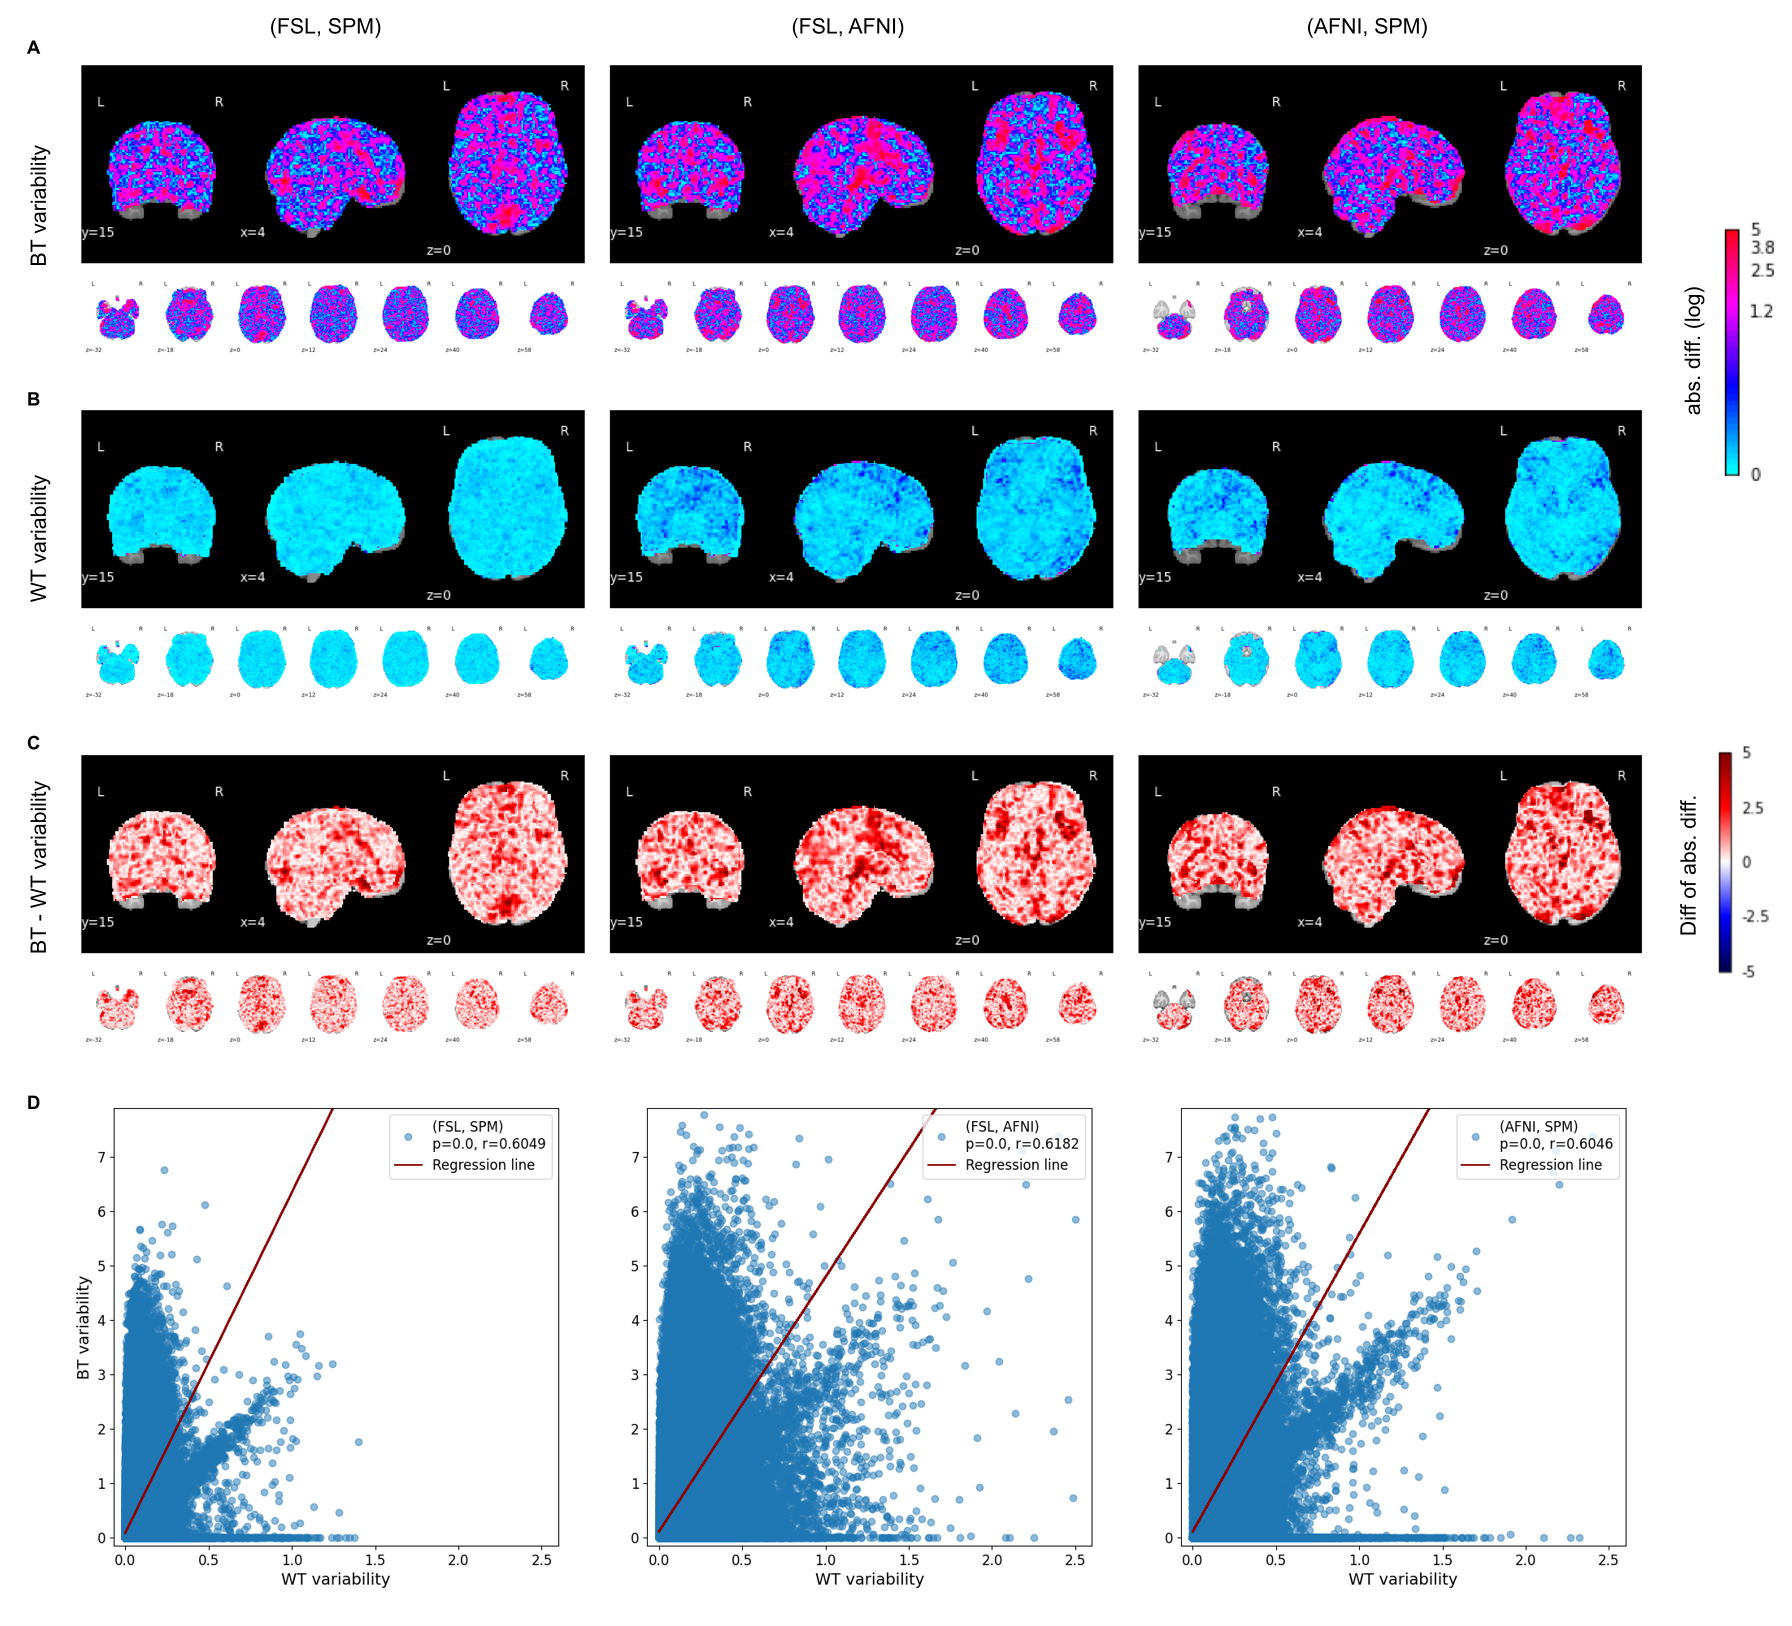
\includegraphics[width=0.9\textwidth]{figures/abs/gl-unthresh.png}
    %\caption{Standard deviation of thresholded t-statistics map on template surface}
  \end{subfigure}
  \caption{Unthresholded group-level variability computed between tools
    (\textbf{A}), within tools at machine error (\textbf{B}), difference
    between them (\textbf{C}), and voxel-wise comparison (\textbf{D}). }
  \label{fig:unthresh-maps}
  % \end{minipage}}
\end{figure*}

\subsection{In subject analyses, WT variability approached BT variability in some regions}

Table~\ref{table:pipeline-stats} also presents summary statistics for
subject-level unthresholded t-statistics maps. As for group-level maps,
BT variability was consistently larger than WT variability (Wilcoxon
signed-rank test and t-test p~\textless~$10^{-5}$ for all tests).
However, Figure~\ref{fig:unthresh-maps-sbj} shows that for
some subjects, WT variability approached %and even surpassed
BT in some regions. As for the group maps, BT and WT
variability appeared moderately correlated for all subjects (R in [0.484,
    0.633], p=0.0 for all subjects, see Supplemental Material~\ref{sec:supp-subjects}).

%%%%%%%%%% Var. of Unthresh sbj05%%%%%%%%
\begin{figure*}[ht]
  \centering
  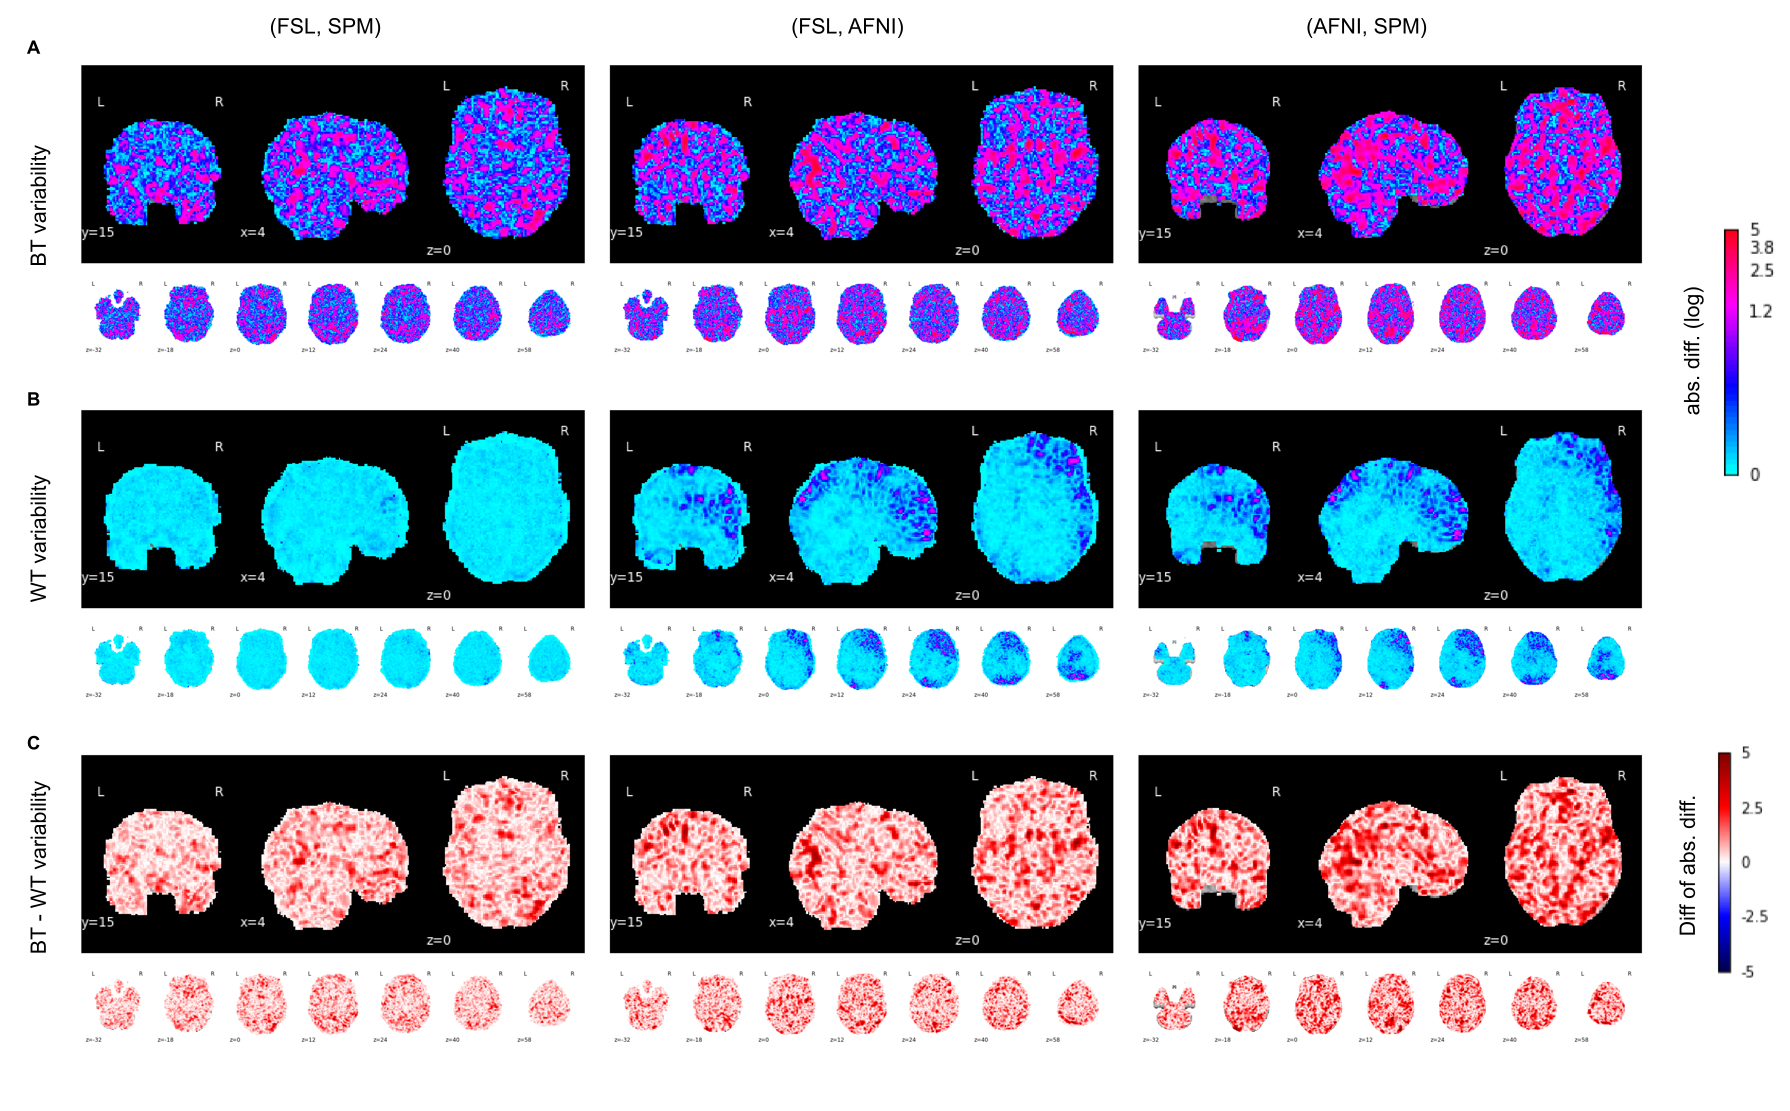
\includegraphics[width=0.9\textwidth]{figures/abs/sbj05-abs.png}
  %\caption{Standard deviation of thresholded t-statistics map on template surface}
  \caption{For subject with highest WT variability,
    unthresholded subject-level variability computed between tools (\textbf{A}), within tools at machine error (\textbf{B}),
    and difference between them (\textbf{C}). \camille{If the changes are visible, I think that it would be useful to add the correspondant unthresholded maps for the reader to see where the differences are and what they "look like"}}
  \label{fig:unthresh-maps-sbj}
\end{figure*}

\subsection{At precision t=17~bits, WT variability approached BT variability in the group analysis}

While the previous results were obtained for machine error, we also
evaluated numerical variability across different virtual precisions for FSL
and found that the virtual precision of t=17 bits minimized the RMSE
between BT and WT in unthresholded group maps.
FSL produced group maps with $\mu=0.483$ and $\sigma=0.410$ at this virtual precision,
which indicates a bit lower variability compared to BT variability
(Wilcoxon signed-rank test and t-test p~\textless~$10^{-5}$ for all tests).
Figure~\ref{fig:gnp-mni} shows BT
and WT in the corresponding group maps obtained at t=17 bits, showing that
BT and WT reach comparable magnitudes in some regions. BT and WT remained
moderately correlated at this precision.


%%%%%%%%%% plot different precisions%%%%%%%%
\begin{figure*}[ht]
  \begin{subfigure}[ht]{\textwidth}
    \centering
    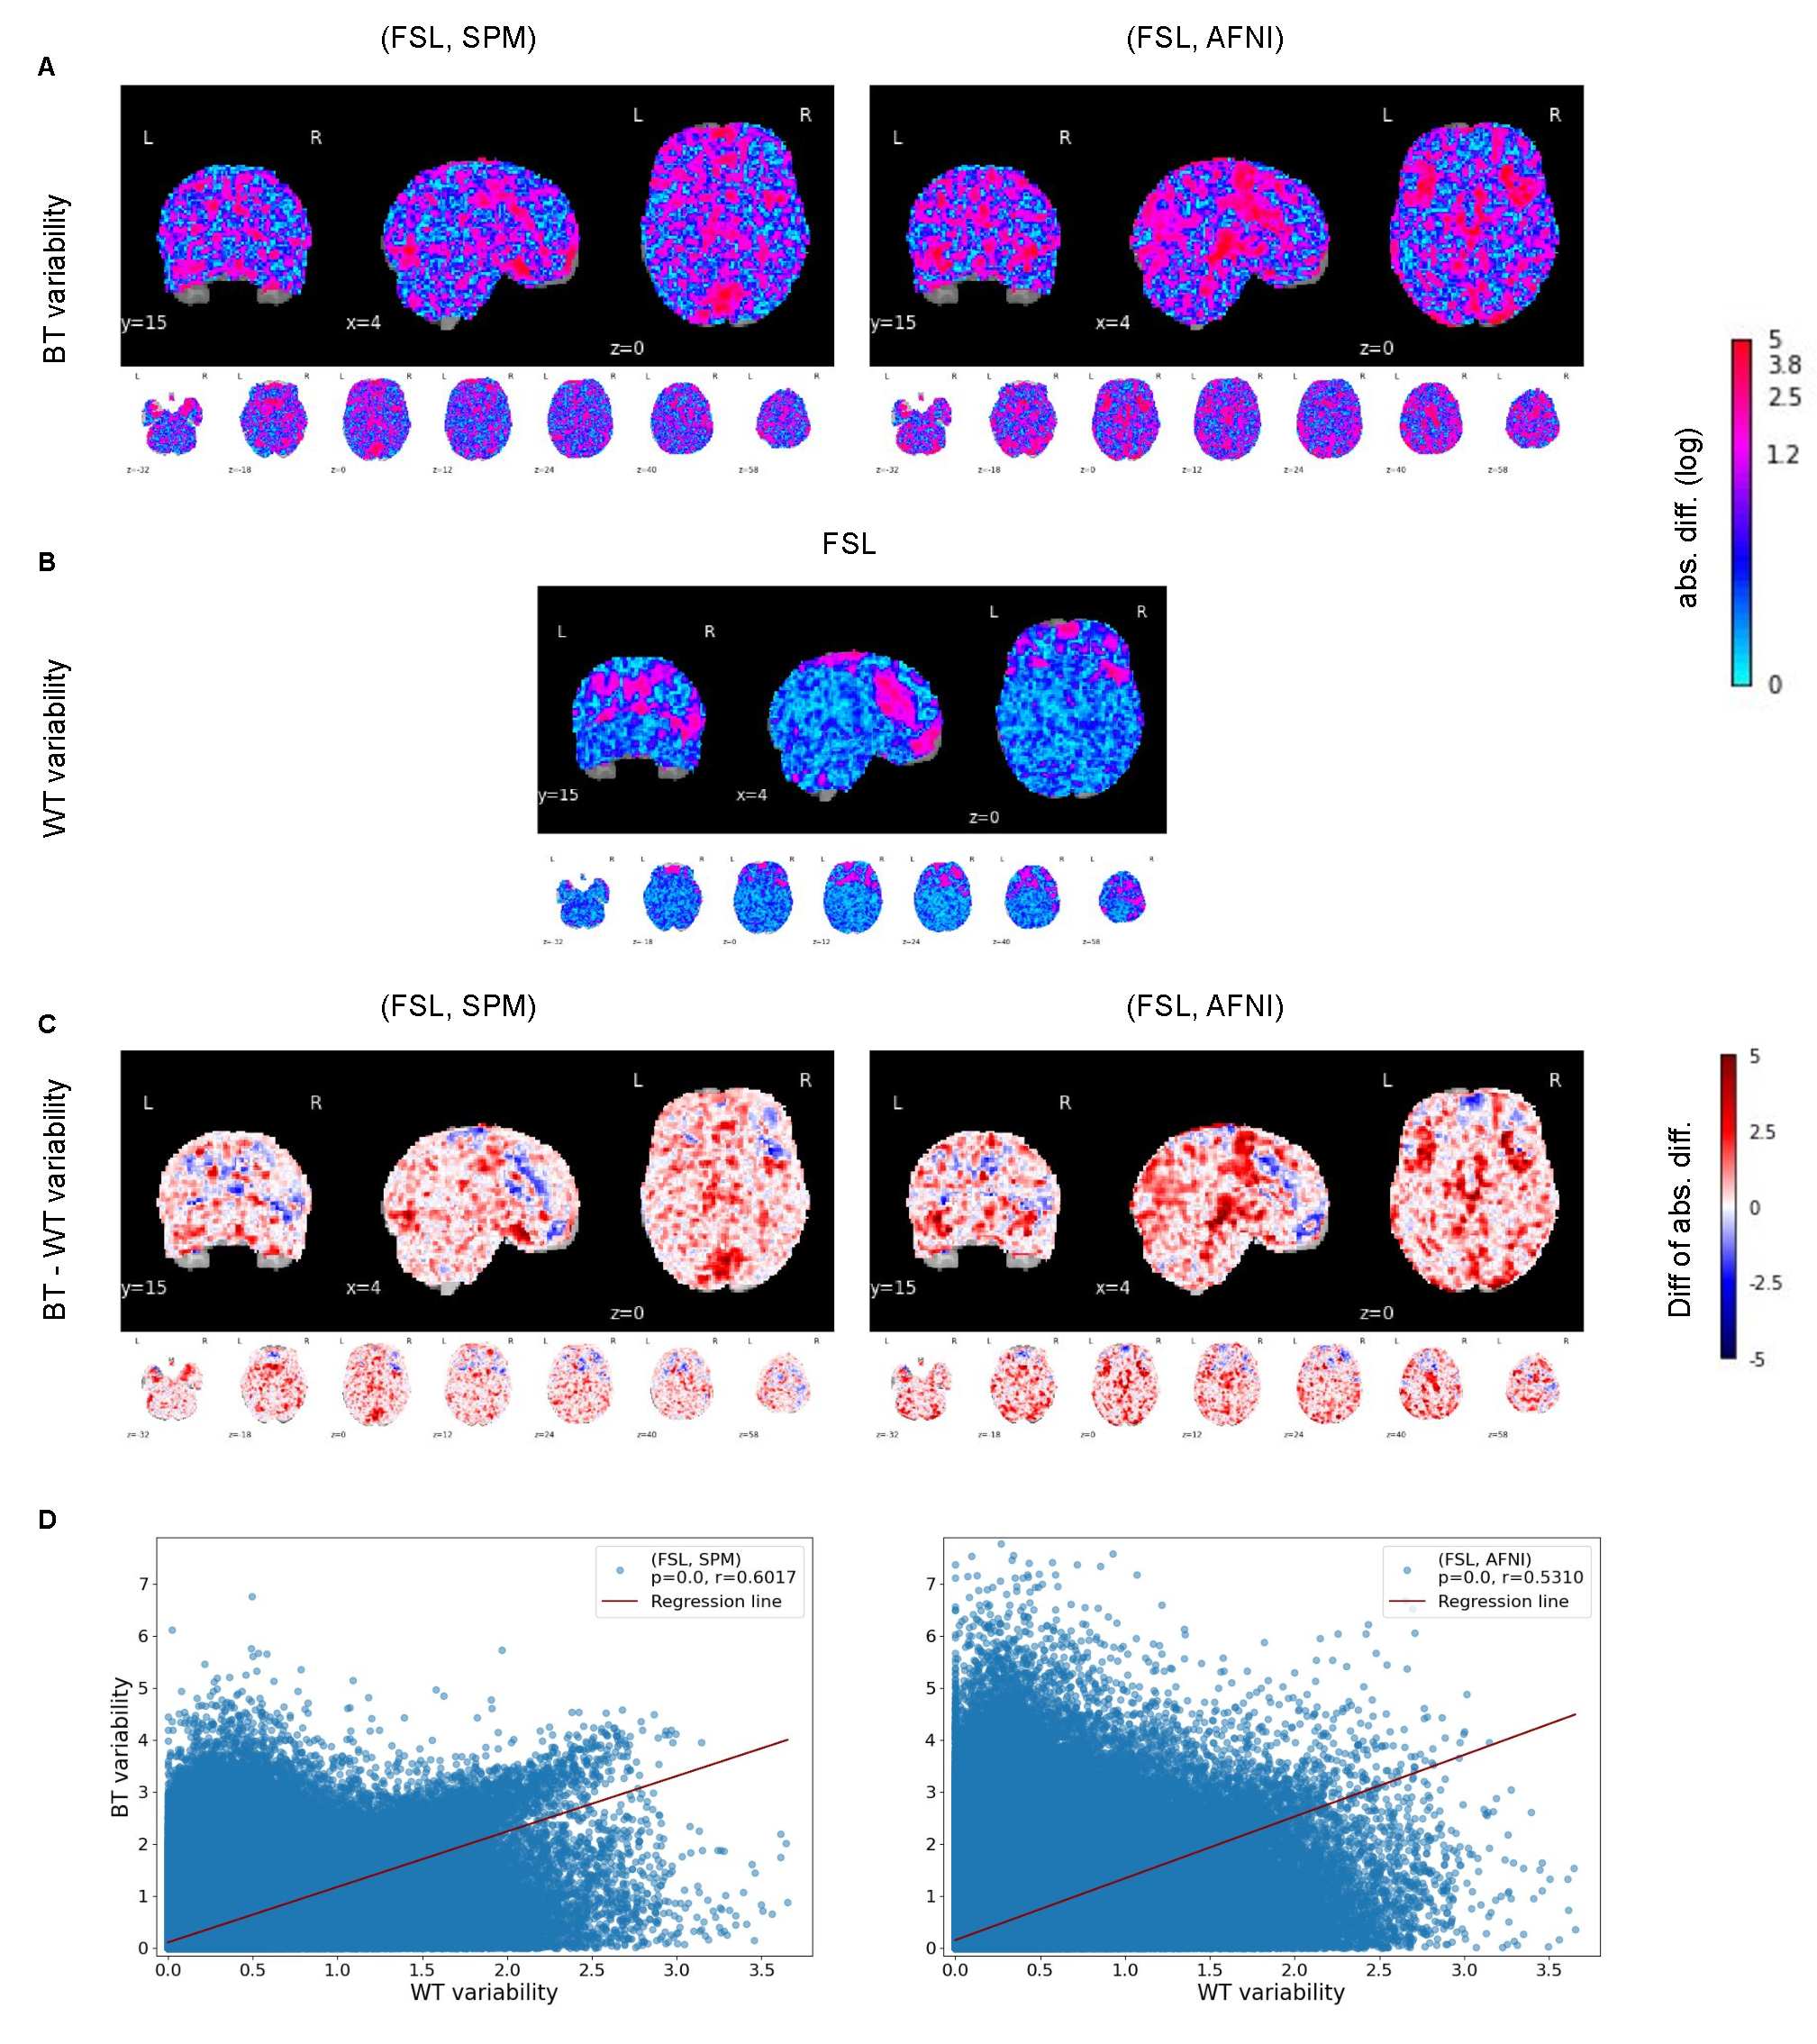
\includegraphics[width=.75\textwidth]{figures/bg_global_precision.pdf}
    %\caption{Standard deviation of thresholded t-statistics map on template surface}
  \end{subfigure}
  %\caption{Standard deviation of thresholded t-statistics map on template surface}
  \caption{Unthresholded group t-statistics absolute differences computed between tools (\textbf{A}),
    within tools at the virtual precision of t=17~bits (\textbf{B}), difference between them (\textbf{C}), and
    voxel-wise comparison (\textbf{D}).}
  \label{fig:gnp-mni}
\end{figure*}


\subsection{Previous results were confirmed in thresholded group maps}

Figure~\ref{fig:thresh-maps}-\textbf{A},\textbf{B},\textbf{C} compares BT
and WT for thresholded group maps. Thresholding is an unstable operation
that introduced variability at the edges of
active regions for both BT and WT. Except in these regions, BT remained consistently larger
than WT \gk{what regions? This kind of came from nowhere}. Moreover, to measure correlation between BT and WT, we
measured WT instability and BT instability in each region of the
HCP-MMP1.0 parcellation \gk{again, it feels kind of abrupt and I'm not really sure what this section is getting at or how it differs from the previous based on these descriptions. Perhaps introduce that thresholding is common, but since it makes things discontinuous we study it through aparcellation, etc...}. The confusion matrices in
Figure~\ref{fig:thresh-maps}-\textbf{D} report these instabilities for
the 360 tested regions. The average ratio of unstable regions was 26\%
for BT and 9.2\% for WT, which confirmed that BT variability was larger than machine error.
The average Cohen's kappa score\footnote{$\kappa \leq 0$ denotes chance agreement, $-1 \leq \kappa \leq 1$}
between WT instability and BT instability was $\kappa=0.17$, indicating
a moderate agreement between WT instability and BT instability.

%%%%%%%%%% Var. of Thresh %%%%%%%%
\begin{figure*}[ht]
  \begin{subfigure}[ht]{\textwidth}
    \centering
    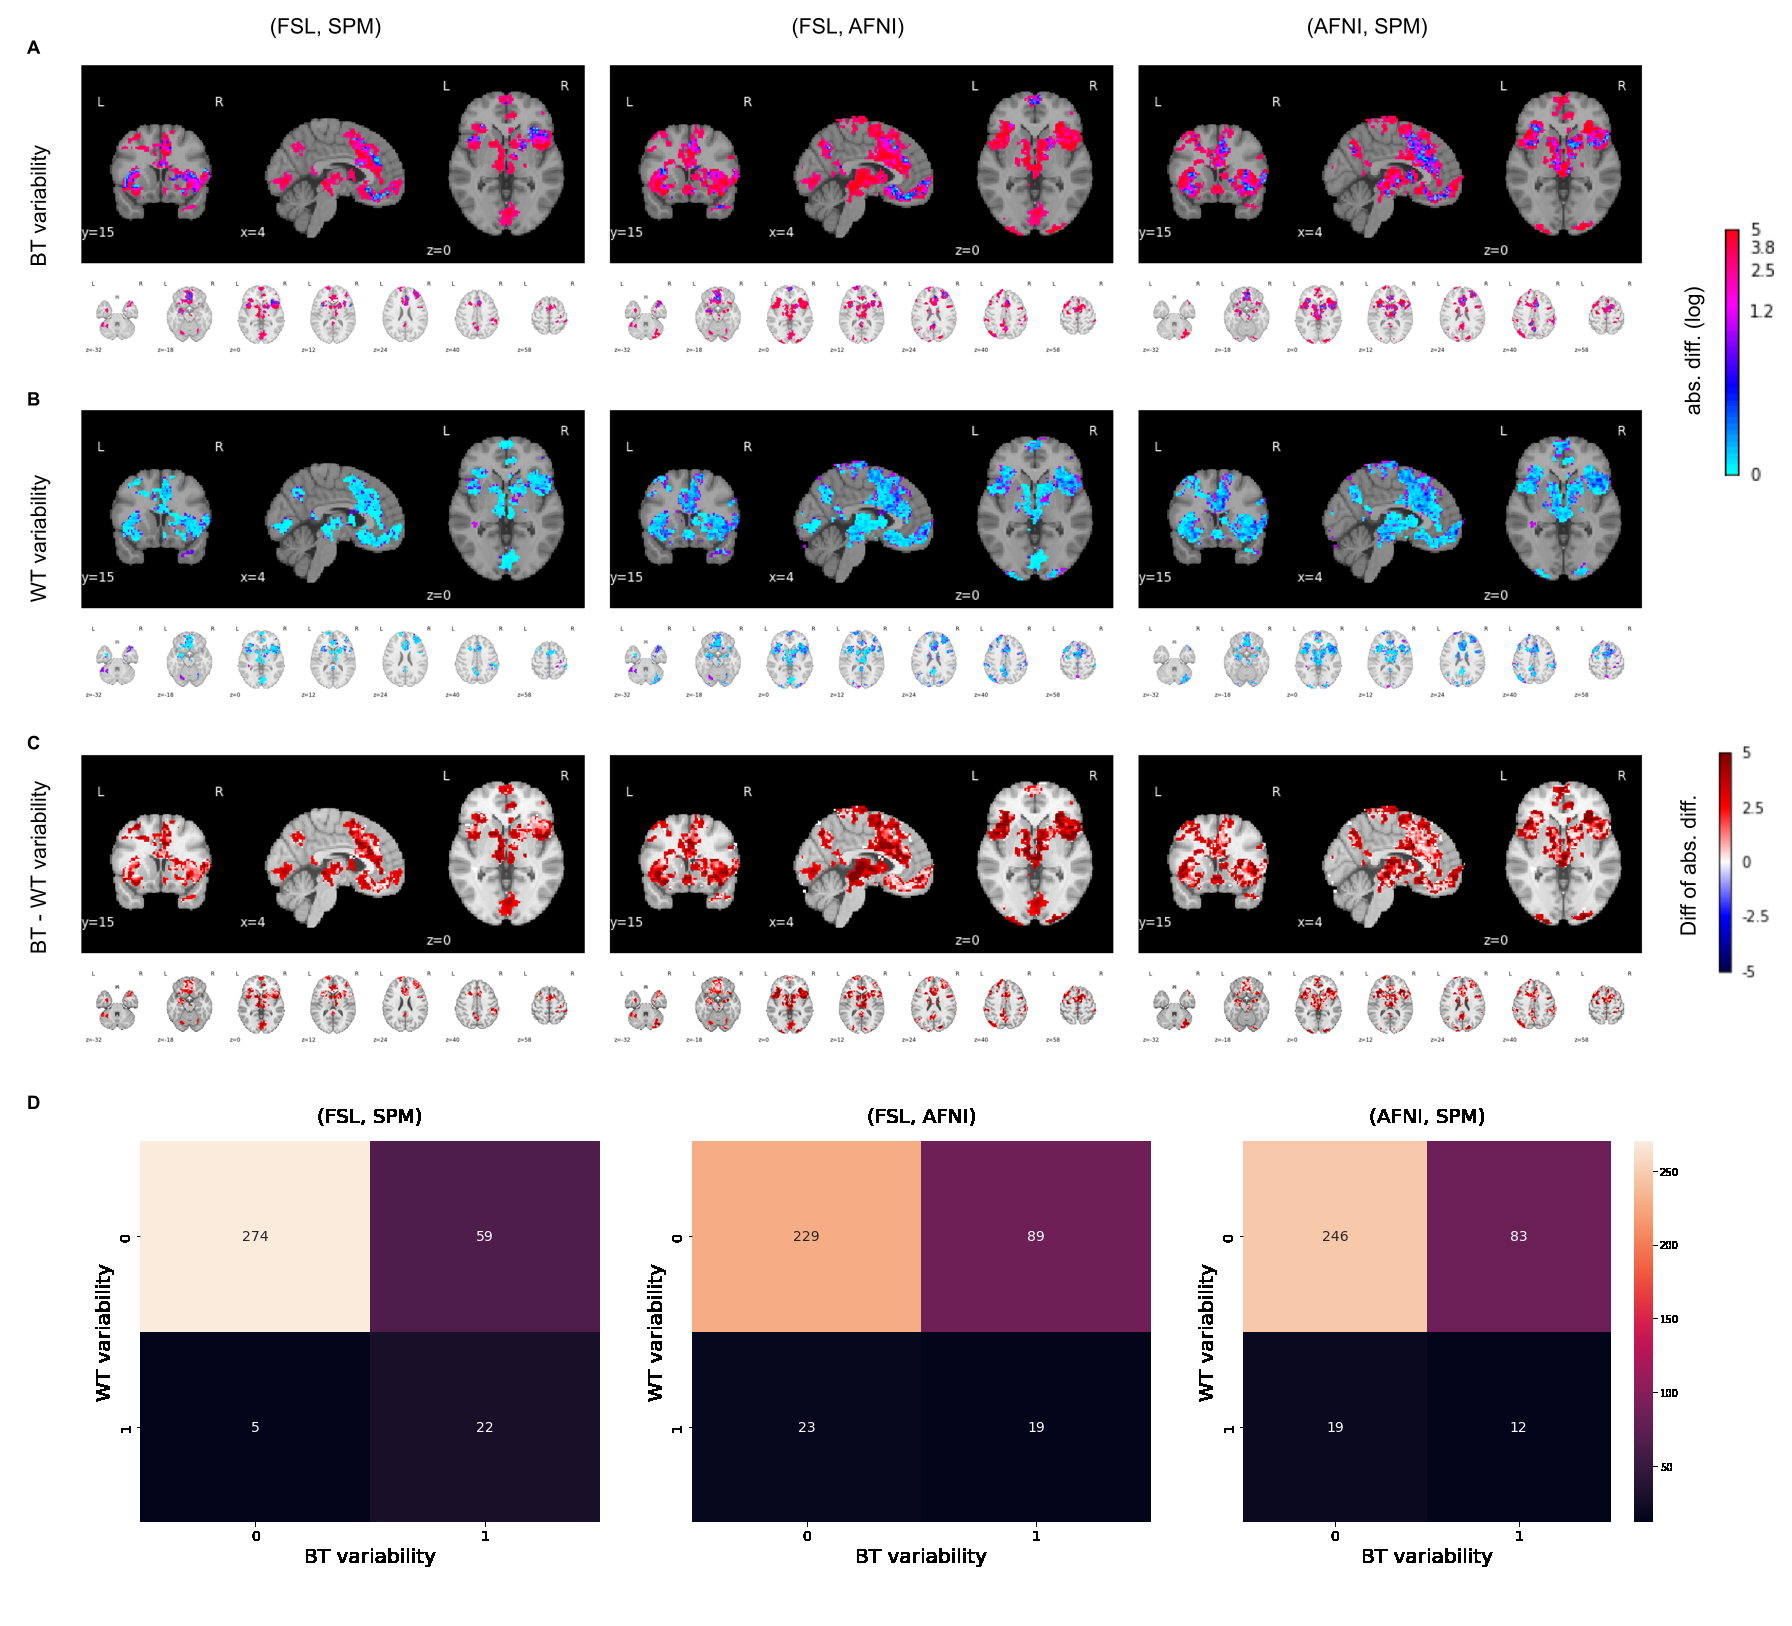
\includegraphics[width=\textwidth]{figures/abs/gl-thresh.png}
    %\caption{Standard deviation of thresholded t-statistics map on template surface}
  \end{subfigure}
  \centering
  \caption{Thresholded group-level variability computed between tools (\textbf{A}),
    within tools at machine error (\textbf{B}), difference between them (\textbf{C}), and
    confusion matrices of activation instability
    in BT and WT among the 360 regions of the HCP-MMP1.0 parcellation (\textbf{D}).}
  \label{fig:thresh-maps}
\end{figure*}


\section{Discussion}

In fMRI group analyses, within-tool variability remains an order of magnitude smaller
than between-tool variability. Group analyses benefit from regularization
of numerical noise, which is expected to increase as sample size
increases. Therefore, for fMRI studies with large sample sizes, within-tool variability may be negligible with respect to between-tool variability. The
recommendation made in~\cite{botvinik2020variability} to rely on
``multiverse'' analyses where multiple analysis tools are compared is
therefore likely to successfully correct for machine error in group
studies. Nevertheless, within-tool variability remains substantial in group analyses
that are based on a single tool, as is commonly the case in current fMRI
studies. In particular, in our study, the inherent instability of
thresholding was triggered by machine error in 9\% of 360 brain regions,
which indicates that machine error might have impacted neuroscientific
conclusions related to these regions.

In subject-level analyses, within-tool and between-tool variabilty can become
of comparable magnitude for some subjects in some regions. This observation
is particularly relevant to the development of fMRI-based biomarkers aiming
at individualized phenotype predictions. Machine error is expected to play
a non-negligible role in such analyses, even when predictions combine
results produced by multiple tools. The observed regularization effect of
group analyses toward numerical noise is consistent with observations made
in~\cite{kiar2020numerical} from diffusion MRI where connectome graph
statistics were found to be substantially unstable at the subject-level
while group distributions remained consistent. \gk{this last sentence feels like it belongs in the previous paragraph, right before mentioning thresholding}

For both group- and subject-level analyses, between-tool variability and within-tool
variability were found to be moderately correlated. Even though between-tool
variability and within-tool  variability are different in nature, this result
suggests that in some cases both sources of variability may have a common
cause that might be related to the conditioning of the BOLD signal
estimation problem \gk{I wouldn't necessarily say it's because of "BOLD signal estimation problem", just "algorithms used to process"} in a specific dataset. Therefore, in some regions,
instabilities of similar magnitude may be triggered by small numerical
perturbations, model variations, or implementation differences. For
instance, the analysis of datasets with high motion may be unstable both
across tools and numerically.

Therefore, numerical stability may be a suitable proxy to study
between-tool variability. This speculation might be of practical value to
address software variability at large given that numerical stability refers
to a consistent mathematical framework whereas between-tool variability
remains more empirical. Likewise, useful quality control metrics may be derived from numerical and between-tool stability.

The finding that numerical variability approached tool variability at the
virtual precision of t=17~bits is interesting too. Indeed, while machine
error generally introduces differences in the order of \yohanmod{1} \yohan{1/2} ulp
\yohan{Are we talking about one arithmetic operation? Or an entire execution?}
--- or
t=53~bits for double-precision values and t=24~bits for single-precision
ones \yohan{I would not mix virtual precision and error measurement}--- common scientific software dependencies introduce larger errors
.
For instance, SciPy's 2D spline interpolation was recently found to be
precise up to t=10~bits~\cite{pytracer} \tristan{Fix ref}
\yohan{Same as previous, I would talk about significance or relative error, or remove the t= and not talk about virtual precision} and might therefore introduce
numerical perturbations leading to errors in the range of between-tool
variability \tristan{Yohan, please check that sentence}. Such high errors
might be triggered by updates in operating systems, Python, MATLAB, and
other software dependencies.
\yohan{The sentence is ok, just a picky point: the SciPy result you cited describes the precision of the spline implementation while at the end you're talking differences due to updates.
  The nuance is that two versions may have a similar precision and so when you udpate your
  system, the difference between both versions is low but each version can be ill-conditionned.}

Our results are limited by the type of numerical noise introduced in the
analyses. We only perturbed the outputs of elementary
mathematical functions while numerical noise could creep in any
floating-point operation. Our estimation of numerical variability should
therefore be considered a lower bound. Our estimation of tool varability is
also likely to be underestimated, having tested only 3 analytical pipelines
among the thousands available~\cite{carp2012plurality}.

In conclusion, our results motivate further numerical stability
investigations in fMRI analysis pipelines. Pipeline-level analyses could be
conducted to identify specific components that contribute to numerical
variability, and if possible correct them accordingly. When instability is
inherent to the analysis, sampling results distributions through numerical
perturbations might improve stability, as explored in~\cite{kiar2021data}.
Finally, pipeline-specific statistical corrections might be envisaged to
account for numerical variability.

\bibliographystyle{plain}
\bibliography{biblio}

\clearpage

\setcounter{equation}{0}
\setcounter{figure}{0}
\setcounter{table}{0}
\setcounter{section}{0}

\makeatletter
\renewcommand{\theequation}{S\arabic{equation}}
\renewcommand{\thefigure}{S\arabic{figure}}
\renewcommand{\thesection}{S\arabic{section}}

\textbf{\centering \Large Supplemental Materials}

\section{Reproduced results}
\label{sec:supp-repro}

Figure~\ref{fig:replication-diff} shows the difference in SPM and AFNI
group analyses maps between the results in~\cite{bowring2019exploring} and
our replication. Numerical perturbations of 1 ulp are likely to have been
introduced by our replication due to the use of GNU/Octave vs MATLAB for SPM
and multithreading for AFNI \camille{Would this be feasible to check?}. However, the group maps remained very similar
overall, which led us to conclude that our results correctly reproduced
the ones in~\cite{bowring2019exploring}.
\begin{figure*}[ht]
  % \fbox{\begin{minipage}{\dimexpr \textwidth-2\fboxsep-2\fboxrule}
  % \centering
  \includegraphics[width=\textwidth]{figures/replication-diffs.png}
  \caption{Differences between reproduced and original results obtained in~\cite{bowring2019exploring}
    of unthresholded group-level t-statistics for SPM (left) and AFNI (right). \camille{it looks like the highest areas of difference in AFNI are due to difference un masking maybe worth noting?}}
  \label{fig:replication-diff}
  % \end{minipage}}
\end{figure*}

\section{BT and WT correlations for all subjects}
\label{sec:supp-subjects}

Figure~\ref{fig:unthresh-correlation-allsbj} plots the relationship between
WT and BT for each subject, showing a consistent moderate correlation between BT and
WT.

\begin{figure*}[ht]
  \centering
  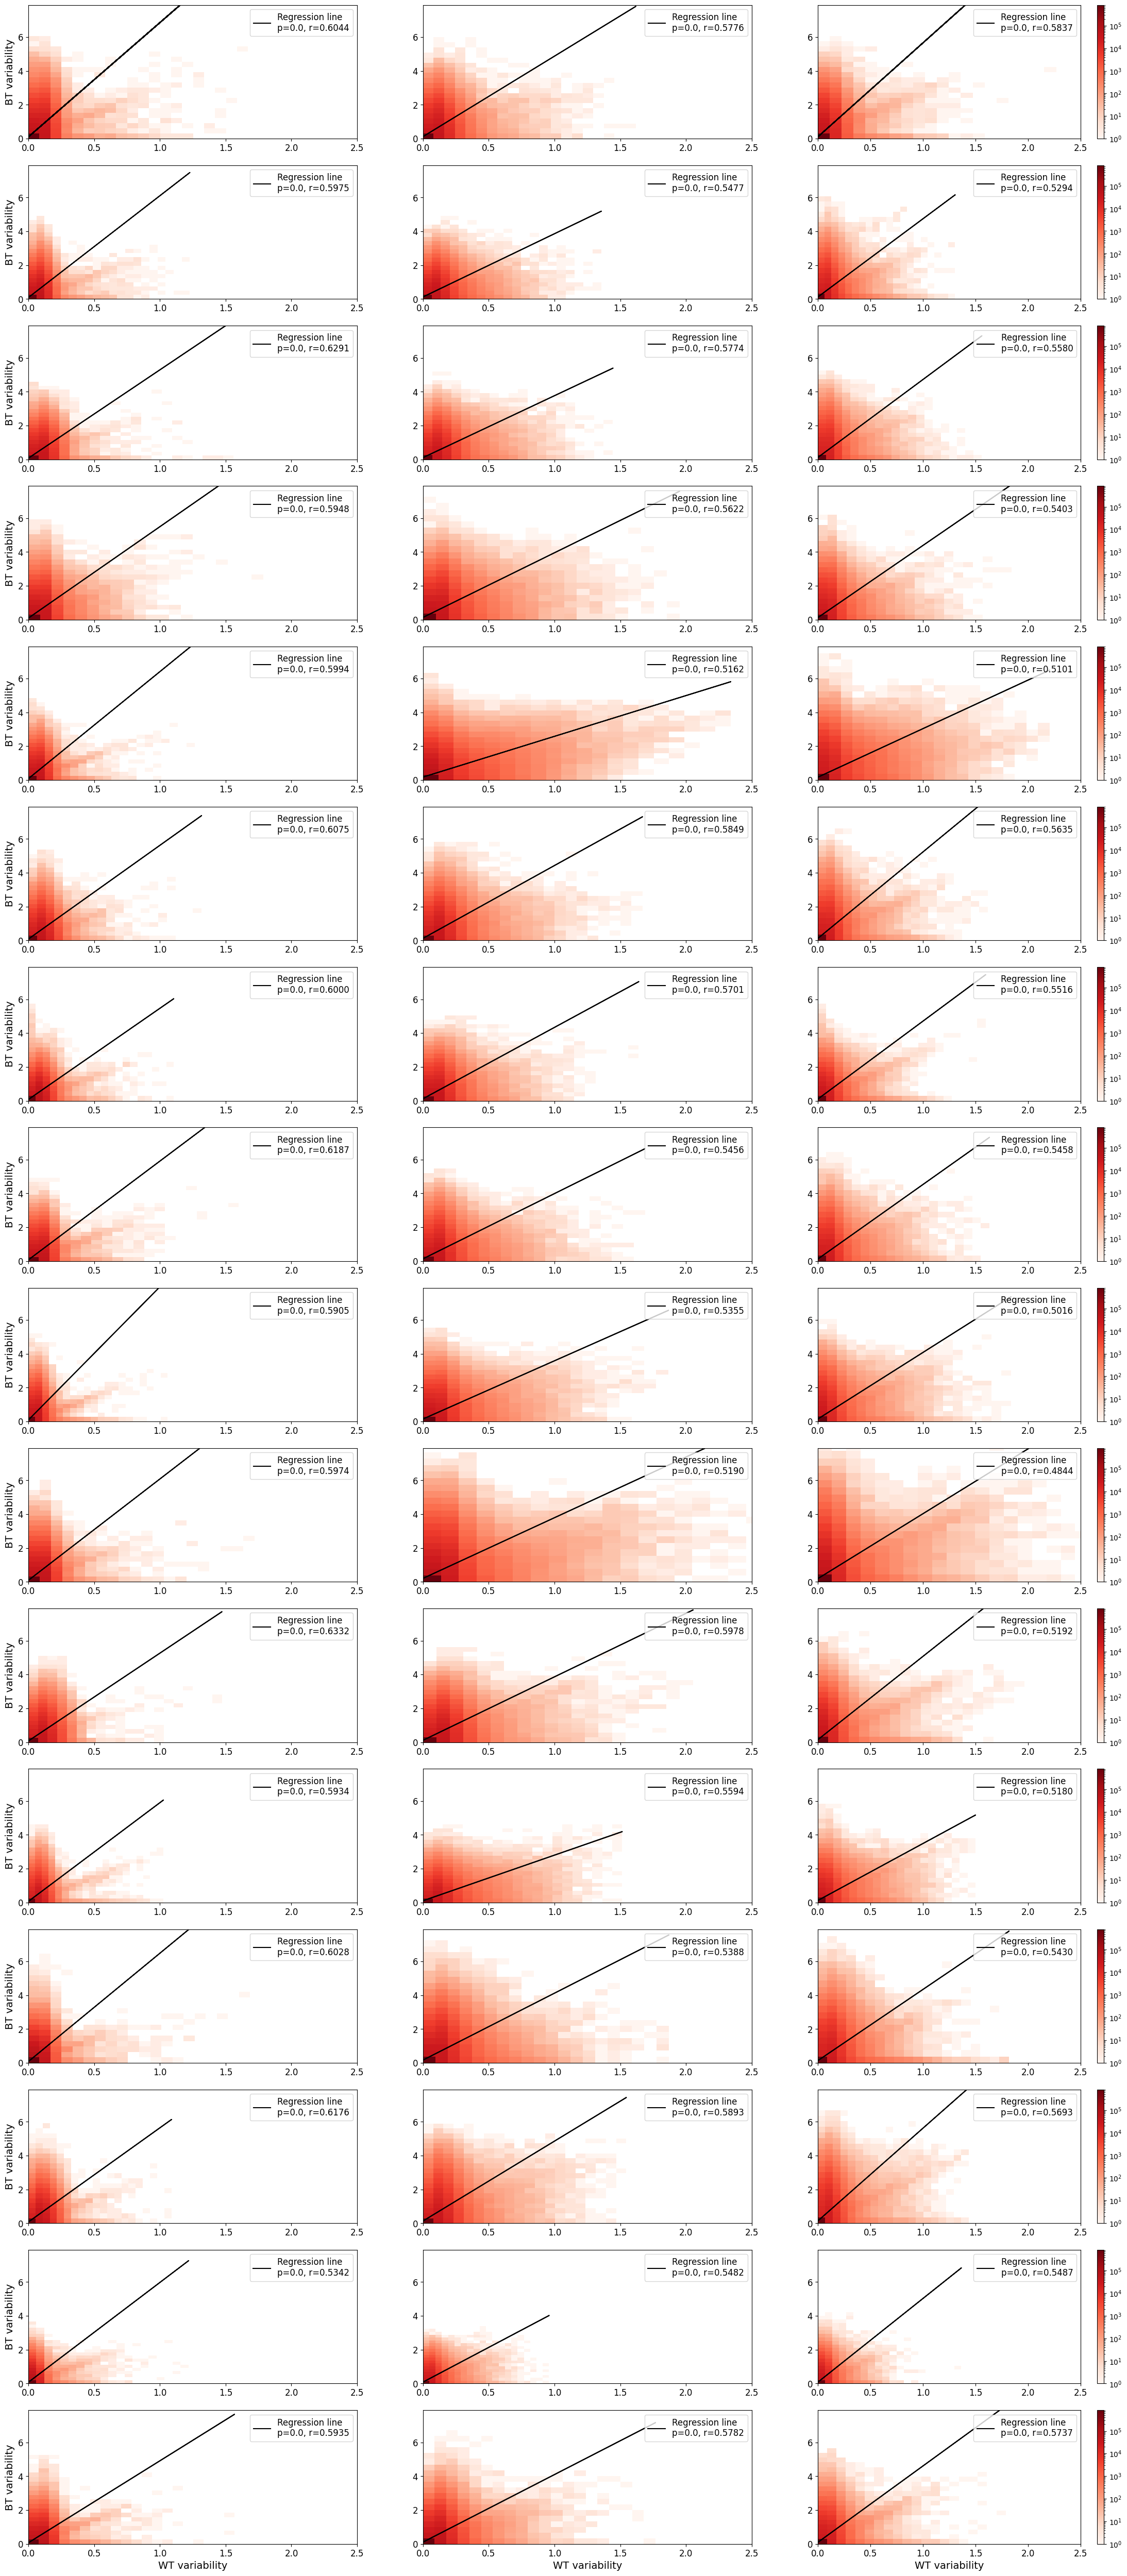
\includegraphics[width=.6\textwidth]{figures/sbj-abs-corr-unthresh-plot.png}
  \caption{Comparison between BT and WT variabilty for 16 subjects.}
  \label{fig:unthresh-correlation-allsbj}
\end{figure*}

\end{document}
\endinput
